\documentclass[11pt]{beamer}
\usetheme{Rochester}

\usepackage[utf8]{inputenc}
\usepackage[T1]{fontenc}

\usepackage{url}

\title{Introduction to Computational Science}
\subtitle{Optimizing Traffic Lights in Urban Street Grids}
\author{Jan Kramer \& Klaas Kliffen}
\setbeamertemplate{navigation symbols}{}

\begin{document}
\maketitle

%dia 1: typen clients
\begin{frame}
\frametitle{Problem introduction}
\begin{columns}
    \begin{column}{.5\textwidth}
        \begin{itemize}
            \item Traffic lights
            \item Long waiting times
        \end{itemize}
    \end{column}
    \begin{column}{.5\textwidth}
        %\begin{figure}
        %\centering
        %\includegraphics[scale=.4]{clients.png}
        %\end{figure}
    \end{column}
\end{columns}
\end{frame}


\begin{frame}
\frametitle{Problem description}
\begin{columns}
    \begin{column}{.5\textwidth}
        \begin{itemize}
            \item Algorithm optimization
            \item Minimize waiting times
            \item Maximize throughput
        \end{itemize}
    \end{column}
    \begin{column}{.5\textwidth}
        %\begin{figure}
        %\centering
        %\includegraphics[scale=.4]{clients.png}
        %\end{figure}
    \end{column}
\end{columns}
\end{frame}

\begin{frame}
\frametitle{Model scope}
\begin{columns}
    \begin{column}{.5\textwidth}
        \begin{itemize}
            \item "American city" grid
            \item Only car traffic (bicycle and pedestrains may be possible too)
            \item No accelartion or decelleration (instant reaction time)
            \item Uniform cars (no buses, trucks etc.)
        \end{itemize}
    \end{column}
    \begin{column}{.5\textwidth}
        %\begin{figure}
        %\centering
        %\includegraphics[scale=.4]{clients.png}
        %\end{figure}
    \end{column}
\end{columns}
\end{frame}

\begin{frame}
\frametitle{Example}

\begin{figure}
\centering
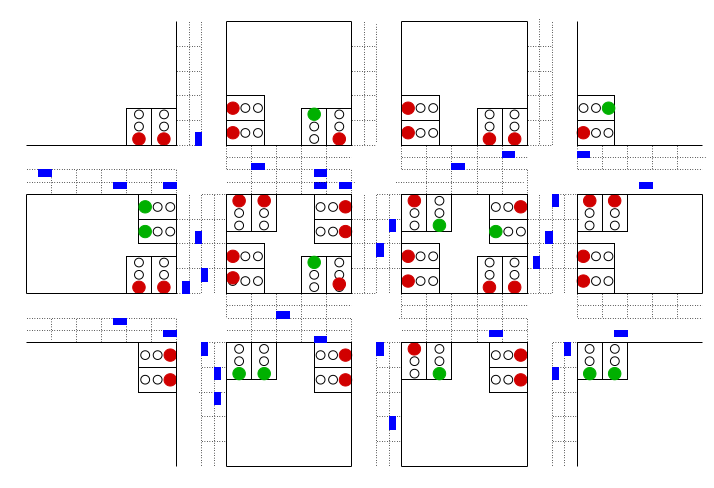
\includegraphics[width=.8\textwidth]{wieringmodel.png}
\caption{Model by Marco Wiering}
\end{figure}
  
\end{frame}

\begin{frame}
\frametitle{Possible traffic light algoritms}
\begin{columns}
    \begin{column}{.5\textwidth}
        \begin{itemize}
            \item Individual timers
            \item Individual loop detection
            \item Globally connected timers or detection
        \end{itemize}
    \end{column}
    \begin{column}{.5\textwidth}
        %\begin{figure}
        %\centering
        %\includegraphics[scale=.4]{clients.png}
        %\end{figure}
    \end{column}
\end{columns}
\end{frame}



\end{document}
